\documentclass[11pt,a4paper,openright,twoside]{report}
\usepackage[utf8]{inputenc}
\usepackage[croatian]{babel}
\usepackage{amsmath, amsfonts, amssymb}
\usepackage{graphicx}
\usepackage{fancyhdr}
\usepackage{color}
\usepackage {tikz}
\usepackage{pgfplots}
\usetikzlibrary {positioning}
\usepackage{tocloft}
\usepackage[hidelinks]{hyperref}
\usepackage[section]{placeins}
\usepackage[final]{pdfpages}
\bibliographystyle{ieeetr}%ieeetr, abbrv
\renewcommand{\cftsecleader}{\cftdotfill{\cftdotsep}}

\usepackage[blocks]{authblk}% The option is for block layout

\newcommand{\kolegij}{}
\newcommand{\naslovRada}{Proračun i konstrukcija 1-stupnjskog reduktora s cilindričnim ravnim zubima \\ {\large Timski projektni zadatak}} 
\newcommand{\mailFriendlynaslovRada}{Konstrukcije - projektni zadatak}

%\author{
%Kristijan Cetina \\{\small JMBAG: 2424011721} \\ {\href{mailto:kcetina@politehnika-pula.hr?subject=\mailFriendlynaslovRada}{{\footnotesize kcetina@politehnika-pula.hr}}} \and 
%Stjepan Grgin \\{\small JMBAG: 0112005802} \\ {\href{mailto:sgrgin@politehnika-pula.hr?subject=\mailFriendlynaslovRada}{{\footnotesize sgrgin@politehnika-pula.hr}}} \and 
%Igor Mrkić \\{\small JMBAG: 0114017089} \\ {\href{mailto:imrkic@politehnika-pula.hr?subject=\mailFriendlynaslovRada}{{\footnotesize imrkic@politehnika-pula.hr}}}
%}


\author[1]{Kristijan Cetina}
\author[2]{Stjepan Grgin}
\author[3]{Igor Mrkić}

\affil[1]{\href{mailto:kcetina@politehnika-pula.hr?subject=\mailFriendlynaslovRada}{kcetina@politehnika-pula.hr} JMBAG: 2424011721}
\affil[2]{\href{mailto:sgrgin@politehnika-pula.hr?subject=\mailFriendlynaslovRada}{sgrgin@politehnika-pula.hr} JMBAG: 0112005802}
\affil[3]{\href{mailto:imrkic@politehnika-pula.hr?subject=\mailFriendlynaslovRada}{imrkic@politehnika-pula.hr} JMBAG: 0114017089}



%\title{\kolegij \\ \naslovRada}
\title{\naslovRada}
\date{Pula, \today}

\begin{document}
\pgfplotsset{width=\textwidth,compat=newest}

\begin{titlepage}
\clearpage
\begin{center}
\begin{Huge}
POLITEHNIKA PULA\\
\end{Huge}
\begin{LARGE}
Visoka tehničko-poslovna škola s p.j.\\
Stručni studij politehnike\\
\end{LARGE}
\end{center}
\vspace{3cm}
{\let\newpage\relax\maketitle}
\thispagestyle{empty}
\vfill
\begin{abstract}
U ovom radu predstavljamo proračun strojnog sklopa - 1-stupanjskog reduktora zajedno s pripradajućim vratilima i ležajevima koji je zadan kao sastavni dio kolegija Konstrukcije.
\end{abstract}
\end{titlepage}
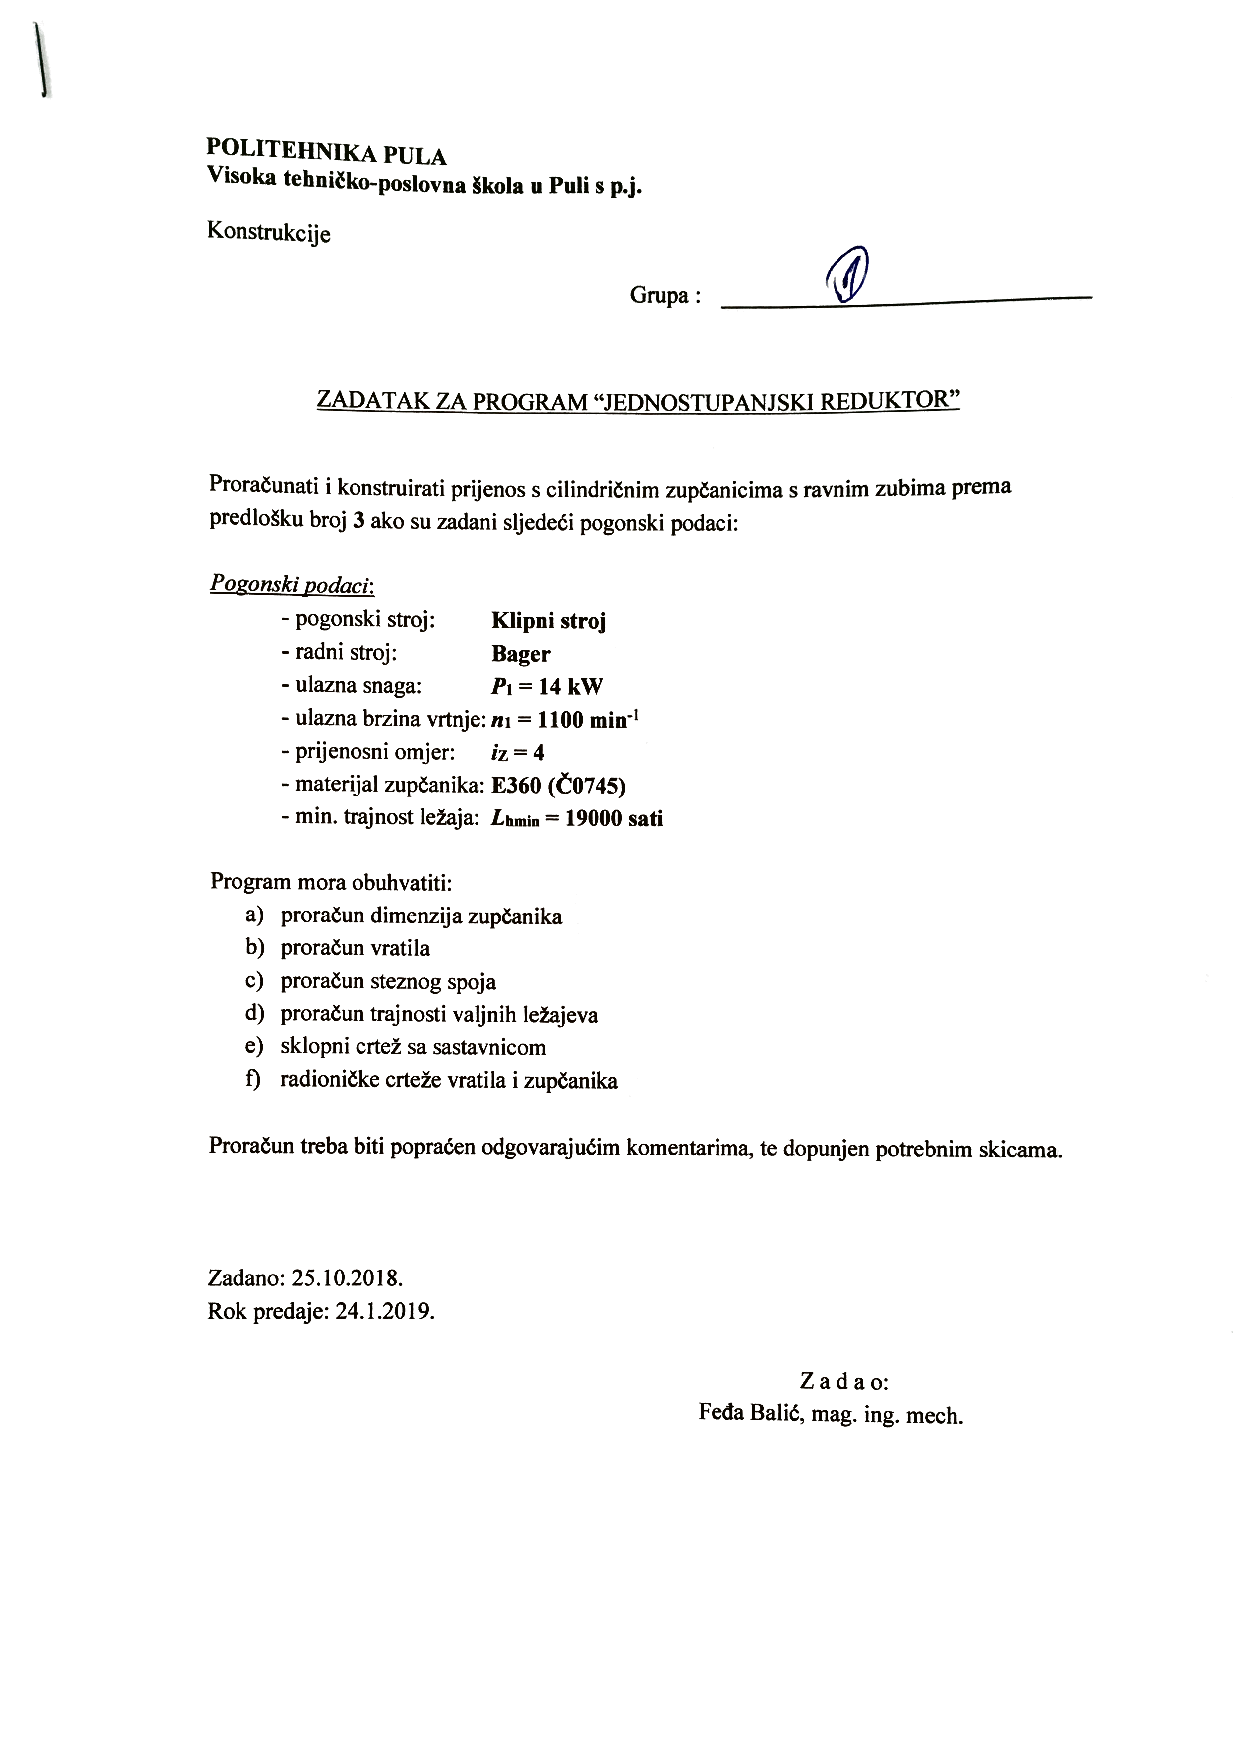
\includepdf[fitpaper]{TimskiProjektniZadatak.pdf}
\tableofcontents
%\listoftables	%ako ih ima puno prebaci na kraj dokumenta
%\listoffigures	%ako ih ima puno prebaci na kraj dokumenta

%Ovdje kreće rad ili može se koristiti
%\input{filename} (da nastavi pisati kako da je copy/paste) ili
%\include{filename} (da ubaci na novu stranicu. Ok za nova poglavlja i sl)
\chapter{Opis zadatka i ograničenja}
\section{Uvod}
Ovaj projektni zadatak nasto je kao obavezni zadatak u sklopu kolegija Konstrukcije koji se održava pod vodstvom Milenka Jokića, dipl.ing., predavača na stručnom studiju politehnike pri Politehnici Pula te asistenciju Feđe Balića, mag. ing. mech.

Prema zadanom predlošku (predložak 3) i zadanim podacima konstriran je 1-stupanjski reduktor s cilindričnim ravnim zubima.
Uvedena su sljedeća pojednostavljena i zanemareni sljedeći dijelovi proračuna:
\begin{itemize}
\item kontrolni pročun
\item izbor ulja za podmazivanje
\item toplinski proračun
\item određivanje stupnja korisnosti
\end{itemize}
Kod proračuna dimenzija zupčanika zanemareni su sljedeći proračuni:
\begin{itemize}
\item nosivost boka zuba
\item sigurnost na \textit{pitting} (površinski zamor)
\item nosivost korjena zuba
\end{itemize}
Kod proračuna vratila izražena je samo kontrola na plastičnu deformaciju te je zanemarena kontrola na zamor materijala.

\chapter{Proračun sklopa}
\section{Proračun dimenzija zupčanika}
Na temelju poznatih pogonskih podatak određen je minimalni diobeni promjer pogonskog zupčanika po izrazu
\begin{equation}
d_1\geq 4045 \cdot \sqrt[3]{\frac{P_1}{\psi_b \cdot n_1} \cdot \frac{i_z +i}{i_z}\cdot K_A \cdot 
K_V \cdot K_{H\alpha} \cdot K_{H\beta} \cdot \left(\frac{S_{Hmin}}{\sigma_{Hlim}}\right)^2 }\label{equ:d1minimalno}
\end{equation}
Pri čemu je $\psi_b=1$ - omjer širine zupčanika i diobenog promjera,
$P_1 \, [kW]$ - snaga pogonskog stroja,
$n_1 \, [s^{-1}]$ - broj okretaja pogonskog stroja,
$i_z$ - željeni prijenosni omjer,
$K_A=2$ - faktor primjene očitan iz tablice \cite{potrebniMaterijali},
$K_V=1$ - faktor dodatnih dinamičkih opterećenja,
$K_{H\alpha}=1$ - faktor raspodjele opterećenja na zube koji su istovremeno u zahvatu,
$K_{H\beta}=1$ - faktor raspodjele opterećenja uzduž boka zuba,
$S_{Hmin}=1,3$ - stupanj sigurnosti na površinski zamor (\textit{pitting}),
$\sigma_{H\lim}=1$ - trajna dinamička čvrstoća boka zuba na kontaktna naprezanja.

Uvrštavanje poznatih podataka u \eqref{equ:d1minimalno} dobije se minimalni diobeni promjer pogonskog zupčanika $$d_1\geq 100,3\,mm$$

Broj zuba pogonskog zupčanika određen je u odnosu na njegovu kutnu brzinu po izrazu
\begin{equation}
\nu=\frac{d_1 \cdot n_1 \cdot \pi}{60}\label{equ:kutnaBrzina}
\end{equation}
Uvrštavanje poznatih podataka u \eqref{equ:kutnaBrzina} dobivena je kutna brzina
$$\nu=5,77 ms^{-1}$$
te je iz tablice \cite{potrebniMaterijali} očitan mogući raspon broja zuba te je usvojen 
$$\mathbf{z_1=21}$$
Broj zuba gonjenog zupčanika je određen
\begin{align*}
z_2&=z_1 \cdot i_z\\
z_2&=21 \cdot 4\\
z_2&=\mathbf{84}
\end{align*}
Stvarni i željeni omjer su isti $$i_z=\mathbf{i_{stv}=\frac{z_2}{z_1}=4}$$
Normalni modul zuba $m_n$ je izračunat:
\begin{align*}
m_n&=\frac{d_1}{z_1}\\
m_n&=\frac{100,3}{21}\\
m_n&=4,776 mm \Rightarrow \mathbf{m_n=5\, mm}
\end{align*}
Razman između osi zupčanika $a$ je određen:
\begin{align*}
a&=\frac{m_n}{2} \cdot (z_1 + z_2)\\
a&=\frac{5}{2} \cdot 105\\
a&=\mathbf{262,5\,mm}
\end{align*}
Stvarni diobeni promjer pogonskog zupčanika izračunat je u ods+nosu na normalni modul i ranije određen broj zuba
\begin{align*}
d_1&=m_n \cdot z_1\\
d_1&=5 \cdot 21\\
d_1&=\mathbf{105 \, mm}
\end{align*}
Širina gonjenog zupčanika:
\begin{align*}
b_2&=\psi_b \cdot d_1\\
b_2&=1 \cdot 105\\
b_2&=\mathbf{105 \,mm}
\end{align*}
Širina pogonskog zupčanika je uvećana za 5 mm u odnosu na gonjeni zupčanik radi aksijalnih pomaka
\begin{align*}
b_1&=b_2+5\,mm\\
b_1&=\mathbf{110 \,mm}
\end{align*}
Diobeni promjer gonjenog zupčanika:
\begin{align*}
d_2&=m_n \cdot z_2\\
d_2&=5 \cdot 84\\
d_2&=\mathbf{420 \,mm}
\end{align*}
Zahvatni kut između zupčanika je odabran standardni kut $\mathbf{\alpha_n=20^\circ}$.
Radijalna zračnost:
\begin{align*}
c&=c^* \cdot m_n\\
c&=0,25 \cdot 5\\
c&= \mathbf{1,25 \, mm}
\end{align*}
Visina korijena zuba:
\begin{align*}
h_f&=m_n+c\\
h_f&=5+1,25\\
h_f&=\mathbf{6,25 \,mm}
\end{align*}
Promjer preko korijena zuba zupčanika:
\begin{align*}
d_{f1}&=d_1-2 \cdot h_f && d_{f2}=d_2-2 \cdot h_f\\
d_{f1}&=105-2 \cdot 6,25 && d_{f2}=420-2 \cdot 6,25\\
d_{f1}&=\mathbf{92,5 \,mm} && d_{f2}=\mathbf{407,5 \,mm}
\end{align*}
Promjer preko glave zuba zupčanika:
\begin{align*}
d_{a1}&=2 \cdot a - d_{f2} - 2 \cdot c  && d_{a2}=2 \cdot a - d_{f1} - 2 \cdot c\\
d_{a1}&=2 \cdot 262,5 - 407,5 - 2 \cdot 1,25 && d_{a2}=2 \cdot 262,5 - 92,5 - 2 \cdot 1,25\\
d_{a1}&=\mathbf{115 \,mm} && d_{a2}=\mathbf{430 \,mm}
\end{align*}

\section{Proračun sila i momenata na zupčanicima}
Moment na ulaznom vratilu:
\begin{align*}
T_1&=\frac{P_1}{\omega_1}\\
T_1&=\frac{14 \cdot 10^3 \cdot 60}{2 \cdot \pi \cdot 1100}\\
T_1&=\mathbf{121,5 \, Nm}
\end{align*}
Snaga na izlaznom vratilu je umanjena za gubitke u sustavu.
\begin{align*}
P_2&=\prod_{i=1}^{n} \eta_i \cdot P_1\\
P_2&=(0,99 \cdot 0,98 \cdot 0,98) \cdot 14\cdot10^3\\
P_2&=\mathbf{13311 \, W}
\end{align*}
Brzina vrtnje izlaznom vratila $n_2=\dfrac{n_1}{i}=\dfrac{1100}{4}=\mathbf{275 \, min^{-1}}$.
Moment na izlaznom vratilu:
\begin{align*}
T_2&=\frac{P_1}{\omega_1}\\
T_2&=\frac{13311 \cdot 60}{2 \cdot \pi \cdot 275}\\
T_2&=\mathbf{462 \, Nm}
\end{align*}
Obodna sila na zupčanicima:
\begin{align*}
F_{t1}&=\frac{2 \cdot T_1}{d_1} && F_{t2}=\frac{2 \cdot T_2}{d_2}\\
F_{t1}&=\frac{2 \cdot 121,5}{0,105} && F_{t2}=\frac{2 \cdot 462}{0,42}\\
F_{t1}&=\mathbf{2314 \, N} && F_{t2}=\mathbf{2200 \, N}
\end{align*}
Radijalna sila na zupčanicima:
\begin{align*}
F_{r1}&=F_{t1} \cdot \tan \alpha_n && F_{r2}=F_{t2} \cdot \tan \alpha_n \\
F_{r1}&=2314 \cdot \tan 20^{\circ} && F_{r2}=2200 \cdot \tan 20^{\circ} \\
F_{r1}&=\mathbf{842 \, N} && F_{r2}=\mathbf{801 \, N}
\end{align*}
Rezultantna sila na zupčanicima:
\begin{align*}
F_1&=\sqrt{F_{t1}^2+F_{r1}^2} && F_2=\sqrt{F_{t2}^2+F_{r2}^2}\\
F_1&=\sqrt{2314^2+842^2} && F_2=\sqrt{2200^2+801^2}\\
F_1&=\mathbf{2462 \, N} && F_2=\mathbf{2341 \, N}
\end{align*}
S obzirom da su ležajevi jednako udaljeni od središta zupčanika svaki od njih trpi jednaku silu:
\begin{align*}
F_{A1}&=F_{B1}=\frac{F_1}{2} && F_{A2}=F_{B2}=\frac{F_2}{2}\\
F_{A1}&=F_{B1}=\frac{2462}{2} && F_{A2}=F_{B2}=\frac{2341}{2}\\
F_{A1}&=F_{B1}=\mathbf{1231 \, N} && F_{A2}=F_{B2}=\mathbf{1171 \, N}
\end{align*}

\section{Proračun vratila}
\subsection{Preliminarni proračun vratila}
Minimalni potrebni promjer vratila izračunat je pomoću izraza:
\begin{equation}
d\geq \sqrt[3]{\frac{16 \cdot T_n \cdot K_A \cdot S}{\pi \cdot R_{dt0}}}\label{equ_minimalniPromjerVratila}
\end{equation}
Pri čemu je $T_n$ - nazivni okretni moment,
$S$ - faktor sigurnosti u rasponu od 10 do 15 zbog zanemarivanja naprezanja uzrokovanih momentom savijanja kao i nepoznavanja konačnog oblika vratila, koncentracija naprezanja i površinske obrade.
$R_{dt0}$ - trajna ishodišna dinamička čvrstoća materija pri torziji. Očitan iz tablice \cite{krivzan1998osnove}

\subsubsection{Pogonsko vratilo}
Za pogonsko vratilo uvrštavanjem u izraz \eqref{equ_minimalniPromjerVratila} izračunati minimalni promjer je:
\begin{align*}
d&\geq \sqrt[3]{\frac{16 \cdot 121,5 \cdot 10^3 \cdot 2 \cdot 12}{\pi \cdot 260}}\\
d&\geq 38,51 \,mm
\end{align*}

Prema tablici\cite{potrebniMaterijali} standardnih dimenzija krajeva cilindričnog vratila prema normi DIN 748 usvojena je dimenzija \textbf{40x110 DIN 748} ($\phi40k6$).
Maksimalni radijus prijelaza je $r_{max}=1 mm$.

Prema tablici standardnih dimenzija uložnih pera\cite{potrebniMaterijali} po DIN 6885 normi usvojeno je pero $\mathbf{DIN6885-A 12 \times 8 \times 100-E295}$ s dubinom utora u vratilu $t_1=5mm$ i utorom u glavini $t_2=3,3mm$.

Promjer na poziciji ležaja $d_L=d+5mm= \mathbf{45 \,mm}$.
Prema katalogu proizvođača ležajeva\cite{skf} odabran je ležaj \textbf{SKF 6008} s potrebnom dimenzijom oslonca ležaja $44,6 \, mm \leq d_a \leq 49,25 \, mm$ te je odabran $\mathbf{d_a=48mm}$.

\subsubsection{Gonjeno vratilo}
Za gonjeno vratilo uvrštavanjem u izraz \eqref{equ_minimalniPromjerVratila} izračunati minimalni promjer je:
\begin{align*}
d&\geq \sqrt[3]{\frac{16 \cdot 462 \cdot 10^3 \cdot 2 \cdot 11}{\pi \cdot 260}}\\
d&\geq 58,39 \,mm
\end{align*}
Prema tablici\cite{potrebniMaterijali} standardnih dimenzija krajeva cilindričnog vratila prema normi DIN 748 usvojena je dimenzija \textbf{60x140 DIN 748} ($\phi60m6$).
Maksimalni radijus prijelaza je $r_{max}=1,6 mm$.

Prema tablici standardnih dimenzija uložnih pera\cite{potrebniMaterijali} po DIN 6885 normi usvojeno je pero $\mathbf{DIN6885-A 18 \times 11 \times 130-E295}$ s dubinom utora u vratilu $t_1=7mm$ i utorom u glavini $t_2=4,4mm$.

Promjer na poziciji ležaja $d_L=d+5mm= \mathbf{65 \,mm}$.
Prema katalogu proizvođača ležajeva\cite{skf} odabran je ležaj \textbf{SKF 31913} s potrebnom dimenzijom oslonca ležaja $73 \, mm \leq d_a \leq 86 \, mm$ te je odabran $\mathbf{d_a=84mm}$.

\subsection{Kontrolni proračun vratila}

\section{Proračun steznog spoja}

\section{Proračun valjnih ležajeva}
Trajnost ležajeva se može proračunati po izrazu
\begin{equation}
L_{10h}=\left(\frac{C}{F} \cdot f_t \right)^p \cdot \frac{10^6}{60 \cdot n}
\label{equ:trajnostLezaja}
\end{equation}
pri čemu je $C$ - dinamička nosivost ležaja, $p$ - eksponent vijeka trajanja. Za kuglične ležajeve $p=3$, za ostale $p=\dfrac{10}{3}$ i $f_t$ - temperaturni faktor. Za $\vartheta < 150^\circ C \Rightarrow f_t=1$.

Odabrani ležajevi za pogonsko vratilo imaju dinamičku nosivost $C=17,8 \,kN$.
Uvršavanje poznatih podataka u \eqref{equ:trajnostLezaja} dobije se minimalna trajnost ležaja
\begin{align*}
L_{10h1}&=\left(\frac{17800}{1231} \cdot 1 \right)^3 \cdot \frac{10^6}{60 \cdot 1100}\\
L_{10h1}&=\mathbf{45808\, h}
\end{align*}
Odabrani ležaj zadovoljava potrebnu minimalnu trajnost iz zahtjeva.

Odabrani ležajevi za gonjeno vratilo imaju dinamičku nosivost $C=54,7 \,kN$.
Uvršavanje poznatih podataka u \eqref{equ:trajnostLezaja} dobije se minimalna trajnost ležaja
\begin{align*}
L_{10h2}&=\left(\frac{54700}{1171} \cdot 1 \right)^{\dfrac{10}{3}} \cdot \frac{10^6}{60 \cdot 275}\\
L_{10h2}&=\mathbf{22247650\, h}
\end{align*}
Odabrani ležaj zadovoljava potrebnu minimalnu trajnost iz zahtjeva.


\newpage
\nocite{*}
\addcontentsline{toc}{chapter}{Literatura}
\bibliography{literatura}

\newpage
\appendix
\addcontentsline{toc}{chapter}{Dodatak A: Radionički nacrt pogonskog vratila}
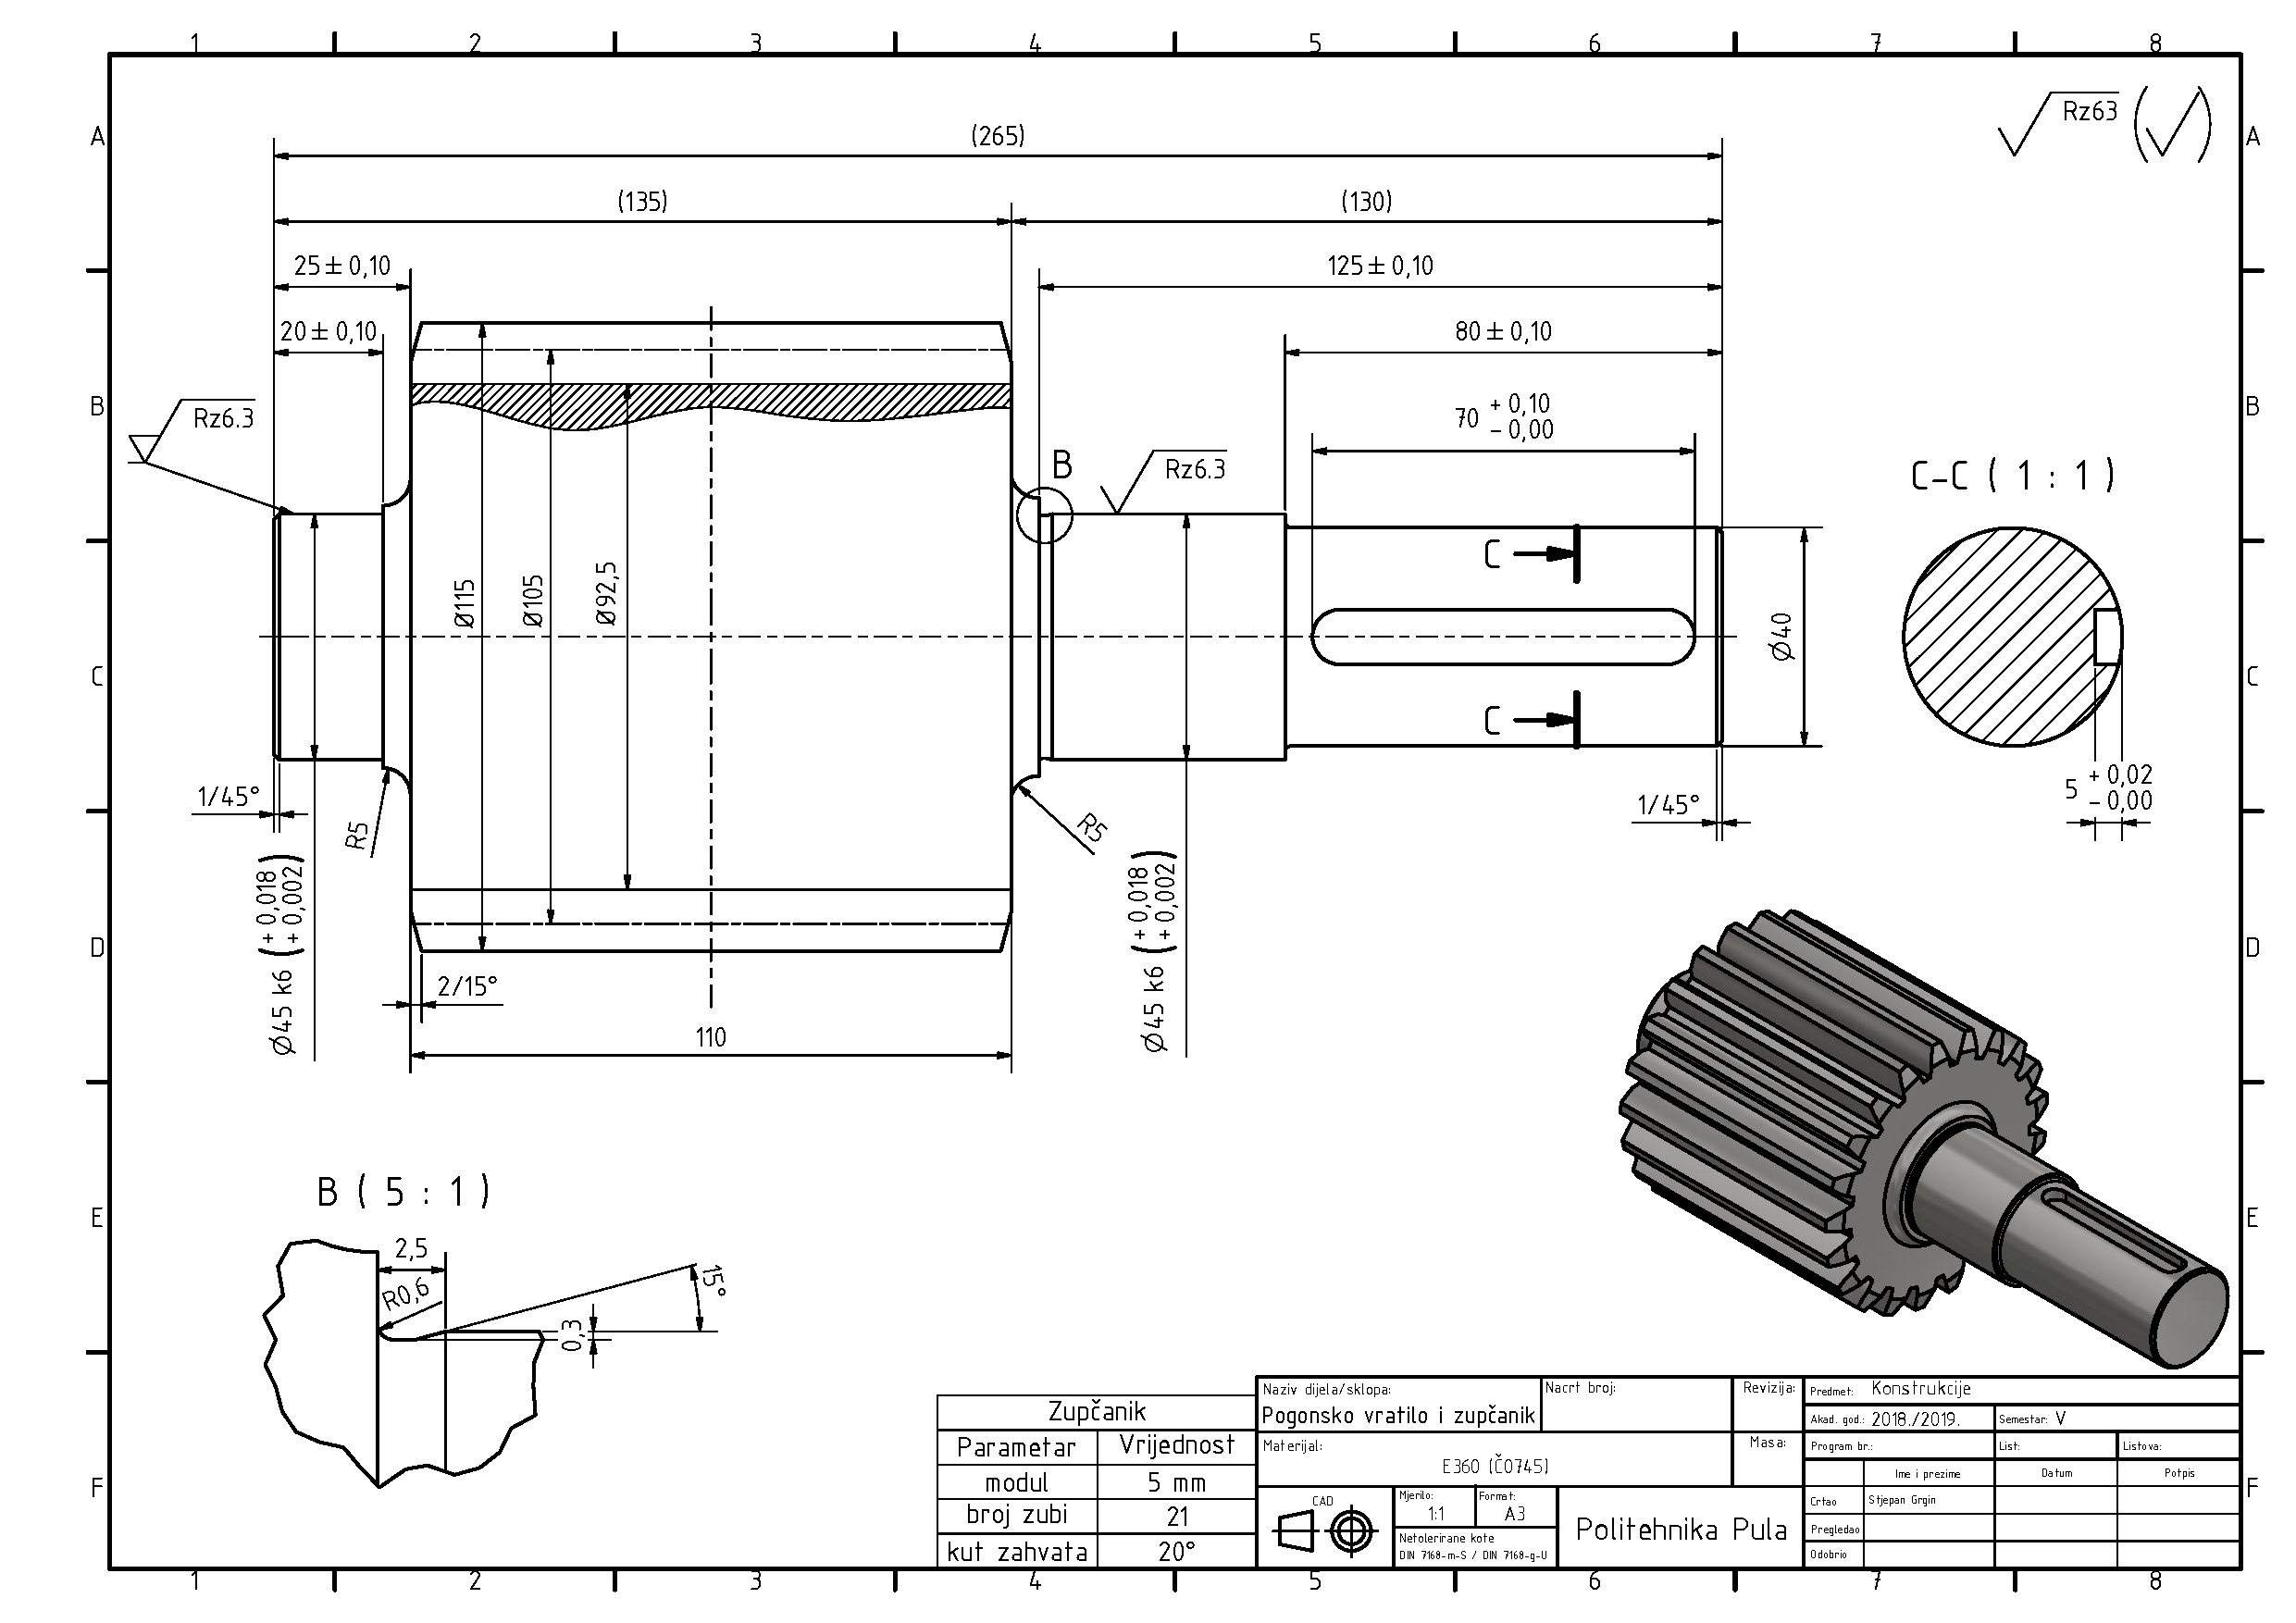
\includepdf[fitpaper]{OutputDrawings/PogonskoVratilo.pdf}
\addcontentsline{toc}{chapter}{Dodatak B: Radionički nacrt gonjenog vratila}
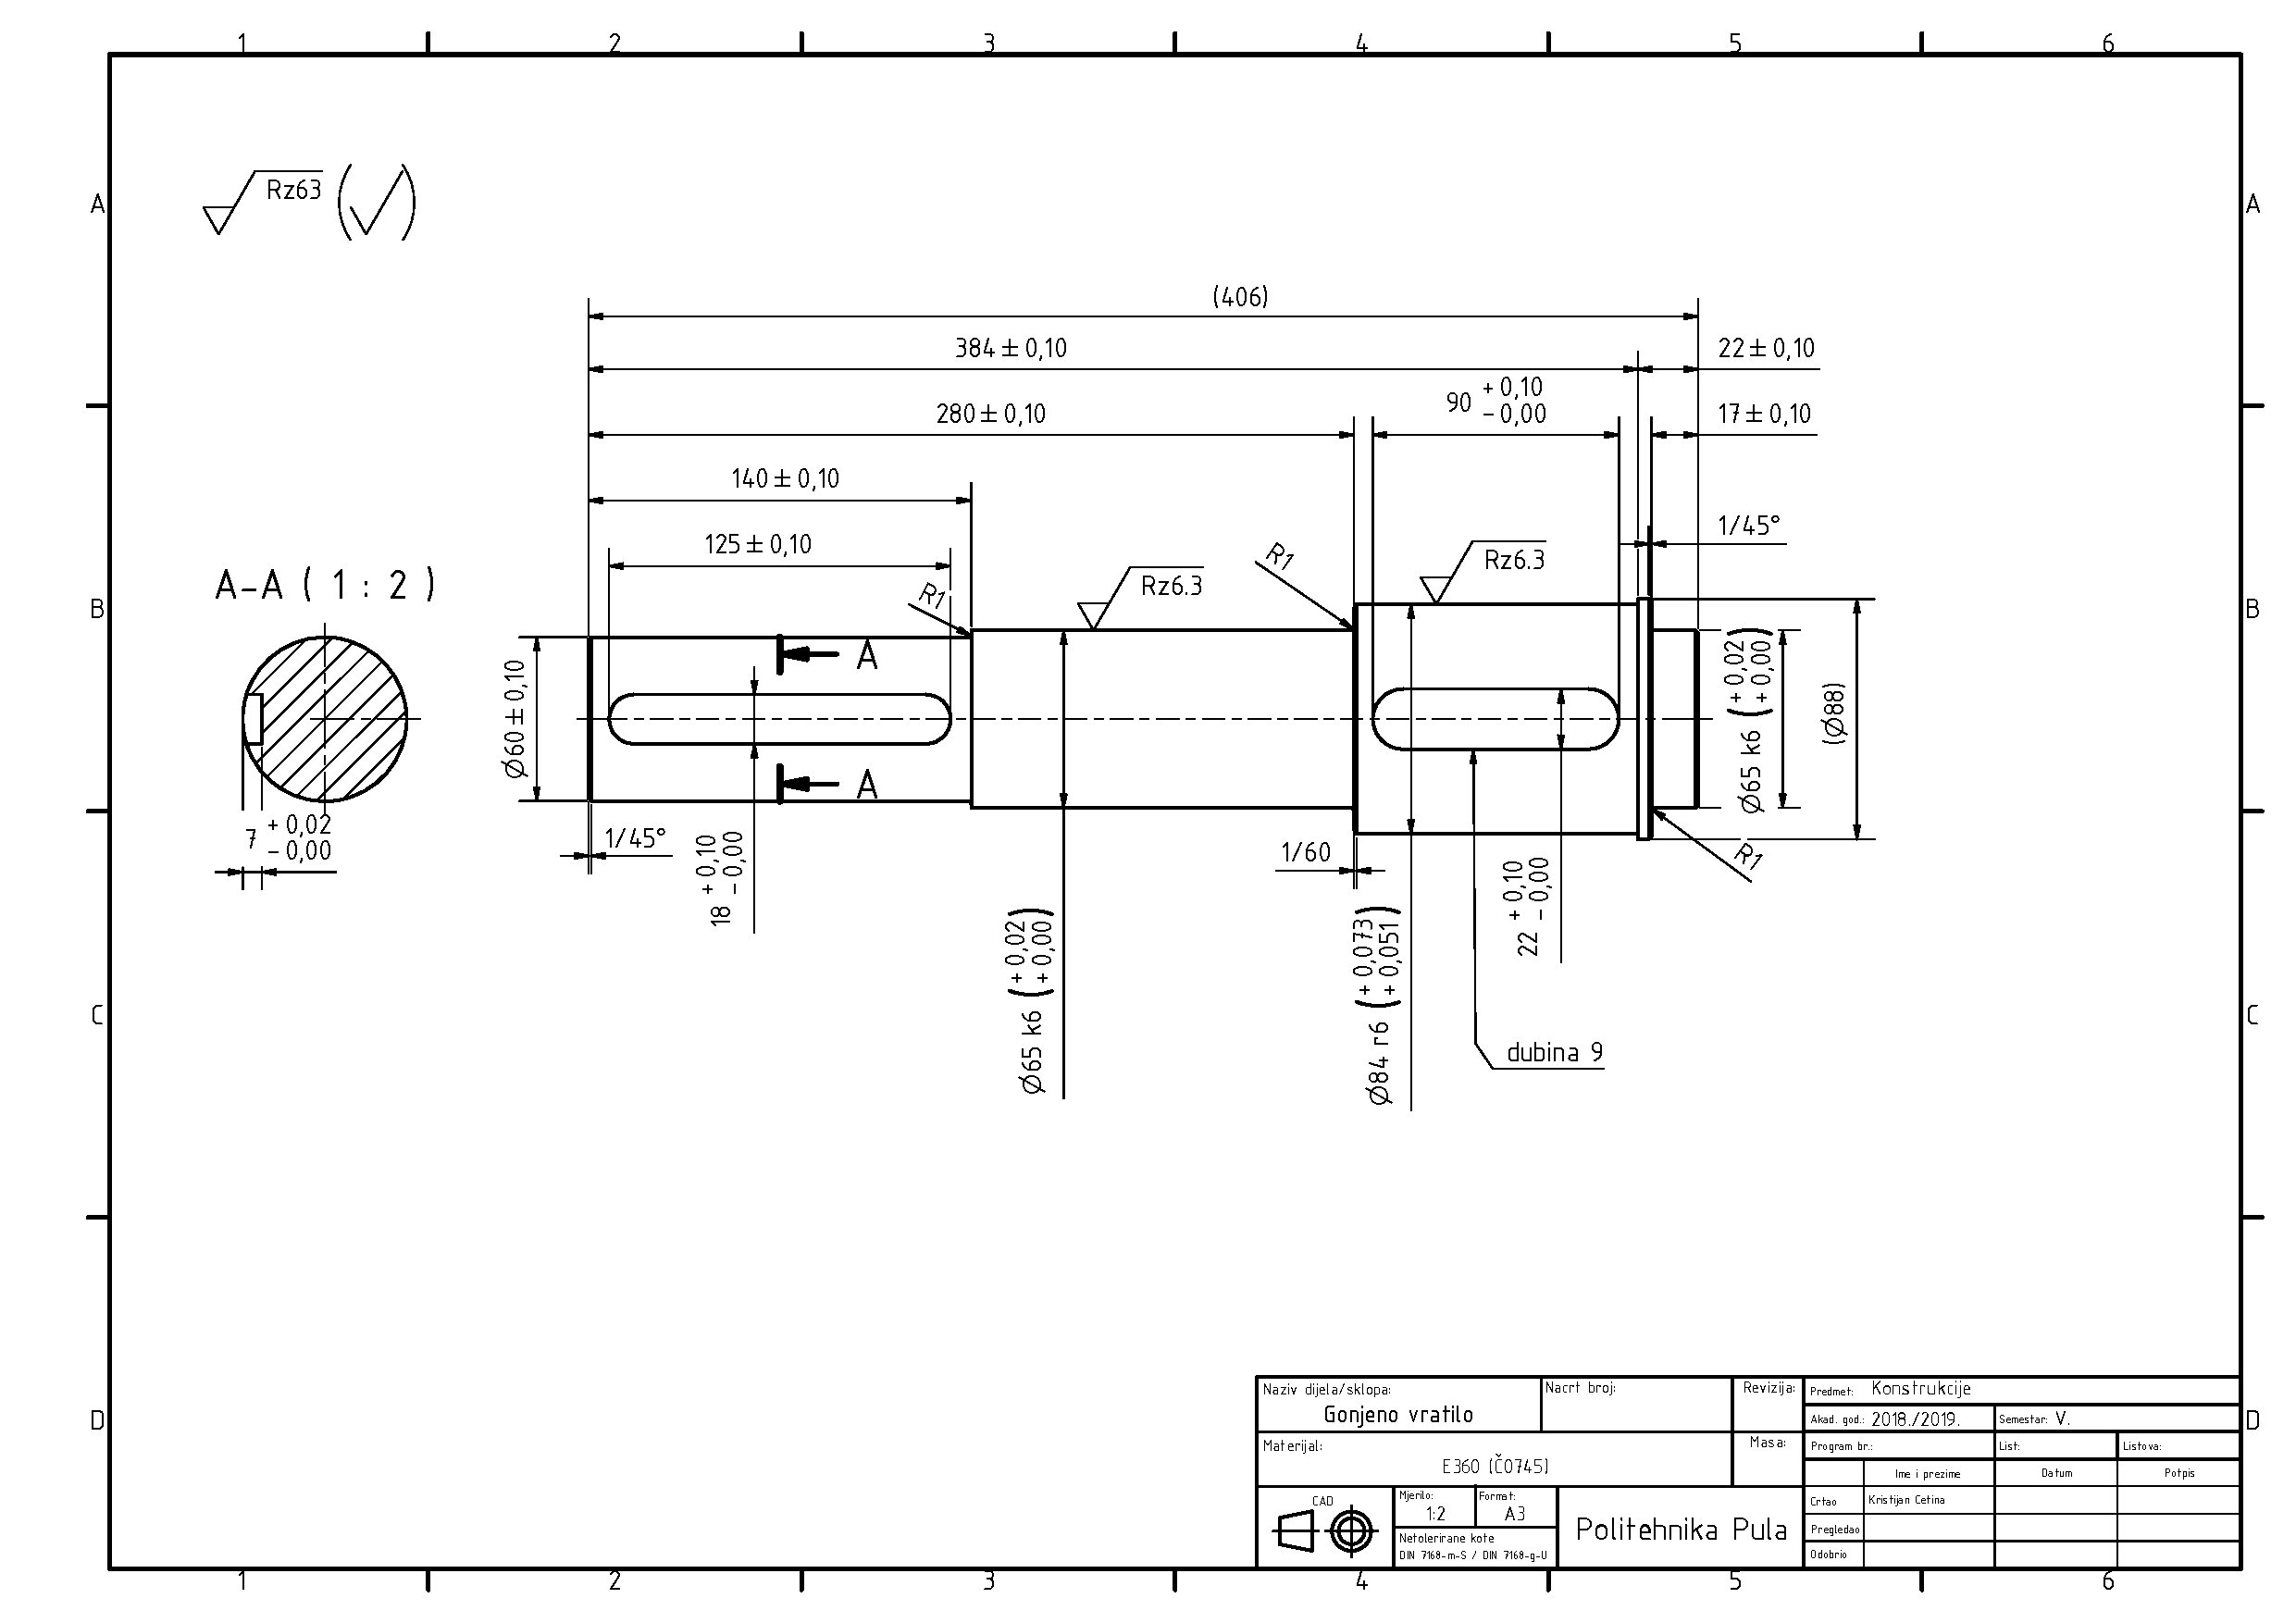
\includepdf[fitpaper]{OutputDrawings/GonjenoVratilo.pdf}
\end{document}